% =====================================================================
%  Atividade Complementar M3 -- Quanto o teste enxerga do pior caso?
%  Sistemas em Tempo Real -- UNIVALI
%  Compilar com pdfLaTeX (padrão do Overleaf).
% =====================================================================
\documentclass[11pt,a4paper]{article}

\usepackage[T1]{fontenc}
\usepackage[utf8]{inputenc}
\usepackage[brazilian]{babel}
\usepackage{lmodern}
\usepackage{textcomp}
\usepackage[a4paper,top=2cm,bottom=2cm,left=2.2cm,right=2cm]{geometry}
\usepackage{setspace}
\usepackage{indentfirst}
\usepackage{amsmath,amssymb}
\usepackage{graphicx}
\usepackage{booktabs}
\usepackage{tabularx}
\usepackage{array}
\usepackage{float}
\usepackage{xcolor}
\usepackage{caption}
\usepackage{enumitem}
\usepackage{microtype}
\usepackage{titlesec}
\usepackage[hidelinks]{hyperref}
\usepackage{url}

\definecolor{univali}{RGB}{31,78,156}
\setstretch{1.05}
\setlength{\parindent}{1.5em}
\titleformat*{\section}{\large\bfseries}
\titleformat*{\subsection}{\normalsize\bfseries}
\titlespacing*{\section}{0pt}{10pt plus 2pt minus 2pt}{5pt}
\titlespacing*{\subsection}{0pt}{7pt plus 2pt minus 2pt}{3pt}
\DeclareCaptionLabelSeparator{travessao}{ --- }
\captionsetup{font=small,labelfont=bf,labelsep=travessao,skip=3pt}
\renewcommand{\topfraction}{0.9}
\renewcommand{\bottomfraction}{0.8}
\renewcommand{\textfraction}{0.07}
\renewcommand{\floatpagefraction}{0.85}
\setcounter{topnumber}{3}
\setcounter{totalnumber}{5}
\setlength{\textfloatsep}{8pt plus 2pt minus 2pt}
\setlength{\floatsep}{6pt plus 2pt minus 2pt}
\setlength{\intextsep}{6pt plus 2pt minus 2pt}
\setlist{itemsep=0pt,topsep=2pt,parsep=0pt}
\newcolumntype{L}{>{\raggedright\arraybackslash}X}

\newcommand{\us}{\ifmmode\,\mu\mathrm{s}\else\,\textmu s\fi}
\newcommand{\ms}{\,ms}
\newcommand{\repositorio}{\url{https://github.com/dibourguignon/str-m3-pior-caso}}

\begin{document}

% =========================== CAPA =====================================
\begin{titlepage}
  \centering
  {\Huge\bfseries\color{univali} UNIVALI\par}
  \vspace{0.5cm}
  {\large Universidade do Vale do Itajaí\par Escola Politécnica\par
   Engenharia de Computação\par Sistemas em Tempo Real\par}
  \vfill
  {\LARGE\bfseries ATIVIDADE COMPLEMENTAR M3\\[2pt]
   QUANTO O TESTE ENXERGA DO PIOR CASO?\par}
  \vspace{0.8cm}
  {\large Codificação de Huffman no ESP32 com FreeRTOS:\\
   tempo de resposta, cobertura e análise $(m,k)$-firme\par}
  \vfill
  {\large\bfseries Acadêmico\par}
  {\large Diego B. Rangel \quad RA: 22.2.1252\par}
  \vspace{0.8cm}
  {\large\bfseries Professores\par}
  {\large Michael Douglas Cabral Alves\par Felipe Viel\par}
  \vspace{0.8cm}
  {\large\bfseries Repositório\par}
  {\large \repositorio\par}
  \vfill
  {\large Itajaí -- SC\par 2026\par}
\end{titlepage}
\setcounter{page}{1}

% ============================ 1 =======================================
\section{Objetivo, plataforma e metodologia}
O trabalho mede o tempo de resposta da mesma tarefa, a codificação de
Huffman~\cite{huffman}, em quatro escopos de teste: tarefa isolada,
comportamental, intertarefas e sistema com carga externa~\cite{enunciado}. A
pergunta é por que o maior tempo observado (HWM) continua subindo depois que a
cobertura do código chega a 100\% e como o modelo $(m,k)$-firme permite
transformar as medições em um critério de teste. O HWM é o máximo de uma
amostra; por isso é um limite inferior do WCRT, e não um valor garantido. A
campanha principal tem 33.000 ativações no ESP32. Como plataforma opcional de
comparação, as mesmas etapas foram executadas em Linux (Seção~\ref{sec:linux}).

\paragraph{Plataforma.} ESP32-D0WD-V3, revisão 3.1, dois núcleos Xtensa LX6,
flash de 4\,MB, CPU fixa em 240\,MHz. O gerenciamento dinâmico de frequência
está desabilitado, então não há \textit{governor}. ESP-IDF 6.0.1 com FreeRTOS
SMP~\cite{espidf}, tick de 1\,kHz, otimização \texttt{-O2} e \textit{watchdog}
de tarefas desligado; Wi-Fi e Bluetooth não são inicializados. As tarefas
medidas ficam presas ao núcleo 1, e o núcleo 0 executa as tarefas do sistema e
os geradores de estímulo. O tick de 1\,kHz foi escolhido porque os intervalos
de 2 a 8\ms{} e os períodos de 4 e 33\ms{} usados nas etapas não existem com a
resolução de 10\ms{} do valor padrão (100\,Hz). No PC (Windows 11) roda apenas
o script de captura em Python, ligado à UART0 (COM3, 115.200 baud), com o
monitor serial fechado.

\paragraph{Entrada e medição.} Código em C. Vetor de $N = 1.024$ caracteres
ASCII imprimíveis (32 a 126), gerado por xorshift64* com semente 20261118, com
distribuição não uniforme (6,2 bits por símbolo depois de codificado). Cada
ativação conta as frequências, monta a árvore com um \textit{min-heap}, gera os
códigos, codifica, decodifica e compara com a entrada. O módulo não usa
\texttt{malloc}. O tempo é lido com \texttt{clock\_gettime(CLOCK\_MONOTONIC)},
com resolução de 1\us; a geração da entrada fica fora do intervalo medido. Os
tempos ficam em RAM e só são enviados ao PC no fim de cada etapa, no formato
\texttt{ativacao,tempo\_us}. Não houve falha de validação em nenhuma ativação.

\paragraph{Deadline e critério comum.} $D = 1{,}2 \times$ HWM(100\%) da
etapa 1 $= 1{,}2 \times 2.265 = 2.718\us$, valor sugerido pelo
enunciado~\cite{enunciado}. O $D$ foi fixado depois da etapa 1 e é o mesmo nas
quatro etapas; apenas o Experimento D usa outros valores. A ativação cumpre o
prazo se $R \le D$. Ativações atrasadas não são descartadas: as liberações
ficam em fila, e o contador de liberações perdidas terminou em zero em todas as
etapas.

\subsection{Etapas: caso, procedimento e critério}
\textbf{1 -- Tarefa.} \textit{Caso:} Huffman isolado (prioridade 10, núcleo 1),
sem outras tarefas da aplicação; 10.000 ativações seguidas, com um vetor novo
gerado antes de cada medição. \textit{Procedimento:} gravar o firmware
(\texttt{esp32/build.ps1 -Upload}) e executar \texttt{esp32/capture.py COM3},
que reinicia a placa e grava os CSV de todas as etapas em sequência. Mede-se da
cópia do vetor ao fim da validação. \textit{Critério:} saída idêntica à
entrada em todas as ativações; o HWM desta etapa define $D$.

\textbf{2 -- Comportamental.} \textit{Caso:} um evento externo por vez. Uma
tarefa no núcleo 0 gera uma borda de subida no GPIO 18, que provoca uma
interrupção no núcleo 1; a rotina de interrupção acorda a tarefa Huffman. O
evento seguinte só é gerado depois da confirmação e de um intervalo aleatório
de 2 a 6\ms. São 3.000 eventos. \textit{Procedimento:} mesmo firmware e mesma
captura. Mede-se do instante da borda ao fim da validação, o que inclui a
interrupção e o despacho. \textit{Critério:} todos os eventos atendidos com
saída correta.

\textbf{3 -- Intertarefas.} \textit{Caso:} três tarefas periódicas no núcleo 1,
liberadas por um timer de hardware de 1\,kHz, com prioridades por taxa
(\textit{rate monotonic}~\cite{liu}): \textit{sensor} (4\ms, prioridade 12,
processa e escreve 128\,B no buffer), \textit{huffman} (10\ms, prioridade 10,
copia o buffer de 1.024\,B) e \textit{logger} (33\ms, prioridade 8, lê o buffer
e retém o mutex por cerca de 1,5\ms). O buffer é protegido por um mutex do
FreeRTOS, que aplica herança de prioridade~\cite{sha}. As três tarefas são
liberadas juntas no primeiro tick. São 10.000 ativações do \textit{huffman}.
\textit{Procedimento:} mesmo firmware. Mede-se do instante ideal de liberação,
calculado pelo timer, até o fim da validação, o que inclui preempção, bloqueio
e latência. \textit{Critério:} saída correta e nenhuma liberação perdida; o
objetivo é provocar perdas por preempção e bloqueio.

\textbf{4 -- Sistema.} \textit{Caso:} etapa 3, mais uma tarefa esporádica de
eventos GPIO (intervalos de 2 a 8\ms, prioridade 11, codifica 256\,B) e a
recepção de tráfego UART vindo do PC. O script envia sem pausa quadros de
262\,B (cabeçalho \texttt{A5 5A}, número de sequência, 256\,B gerados por
\texttt{random.Random(20261118)} e soma de verificação) a 115.200 baud. O
\textit{driver} UART roda no núcleo 1 com limiar de FIFO de 1 byte, ou seja,
uma interrupção por byte (cerca de 11.500 por segundo), e uma tarefa de
prioridade 11 confere cada quadro e codifica os dados. São 10.000 ativações.
\textit{Procedimento:} o firmware avisa o início e o fim da etapa pela serial,
e o script envia quadros nesse intervalo. \textit{Critério:} saída correta,
quadros recebidos sem erro e cargas ativas. A UART foi escolhida por ser o
canal real entre a placa e o PC; o limiar de 1 byte gera o máximo de
interrupções no núcleo das tarefas, e o estímulo é determinístico. O PC enviou
4.457 quadros (1.167.734\,B, a 11.505\,B/s, a taxa máxima da linha) e o ESP32
validou 4.455, sem nenhum corrompido; os dois restantes estavam em trânsito no
fim da etapa. Houve 15.863 eventos GPIO.

% ============================ 2 =======================================
\section{Estatísticas e distribuição dos tempos}

\begin{table}[H]
\centering
\caption{Síntese com $D = 2.718\us$ (fixo). Tempos em \textmu s.}
\label{tab:sintese}
\footnotesize
\setlength{\tabcolsep}{3.4pt}
\resizebox{\textwidth}{!}{%
\begin{tabular}{@{}lccccccccccc@{}}
\toprule
Etapa & Cob.\ L/D (\%) & Mín. & Média & HWM(100\%) & HWM(99\%) & Prazo (\%) & $S$ & $k{=}10$ & $k{=}20$ & $k{=}50$ \\
\midrule
1. Tarefa         & 100 / 100 & 2.169 & 2.223 & 2.265  & 2.251  & 100,00 & -- & (10,10) & (20,20) & (50,50) \\
2. Comportamental & 100 / 100 & 2.198 & 2.237 & 2.344  & 2.264  & 100,00 & -- & (10,10) & (20,20) & (50,50) \\
3. Intertarefas   & 100 / 100 & 3.266 & 3.359 & 3.928  & 3.903  & 0,00   & 1  & (0,10)  & (0,20)  & (0,50) \\
4. Sistema        & 100 / 100 & 4.350 & 7.488 & 15.213 & 11.562 & 0,00   & 1  & (0,10)  & (0,20)  & (0,50) \\
\bottomrule
\end{tabular}}

\vspace{2pt}
\begin{minipage}{\textwidth}\raggedright\scriptsize
Cobertura de linhas/desvios de \texttt{huffman.c}, medida com gcov no PC sobre o mesmo arquivo usado no firmware (Seção~\ref{sec:expA}). HWM(99\%): máximo depois de retirar o 1\% maior das medições. $S$ em ativações; ``--'' indica menos de duas perdas. Desvios-padrão: 13, 12, 118 e 1.769\us.
\end{minipage}
\end{table}

\begin{figure}[H]
\centering
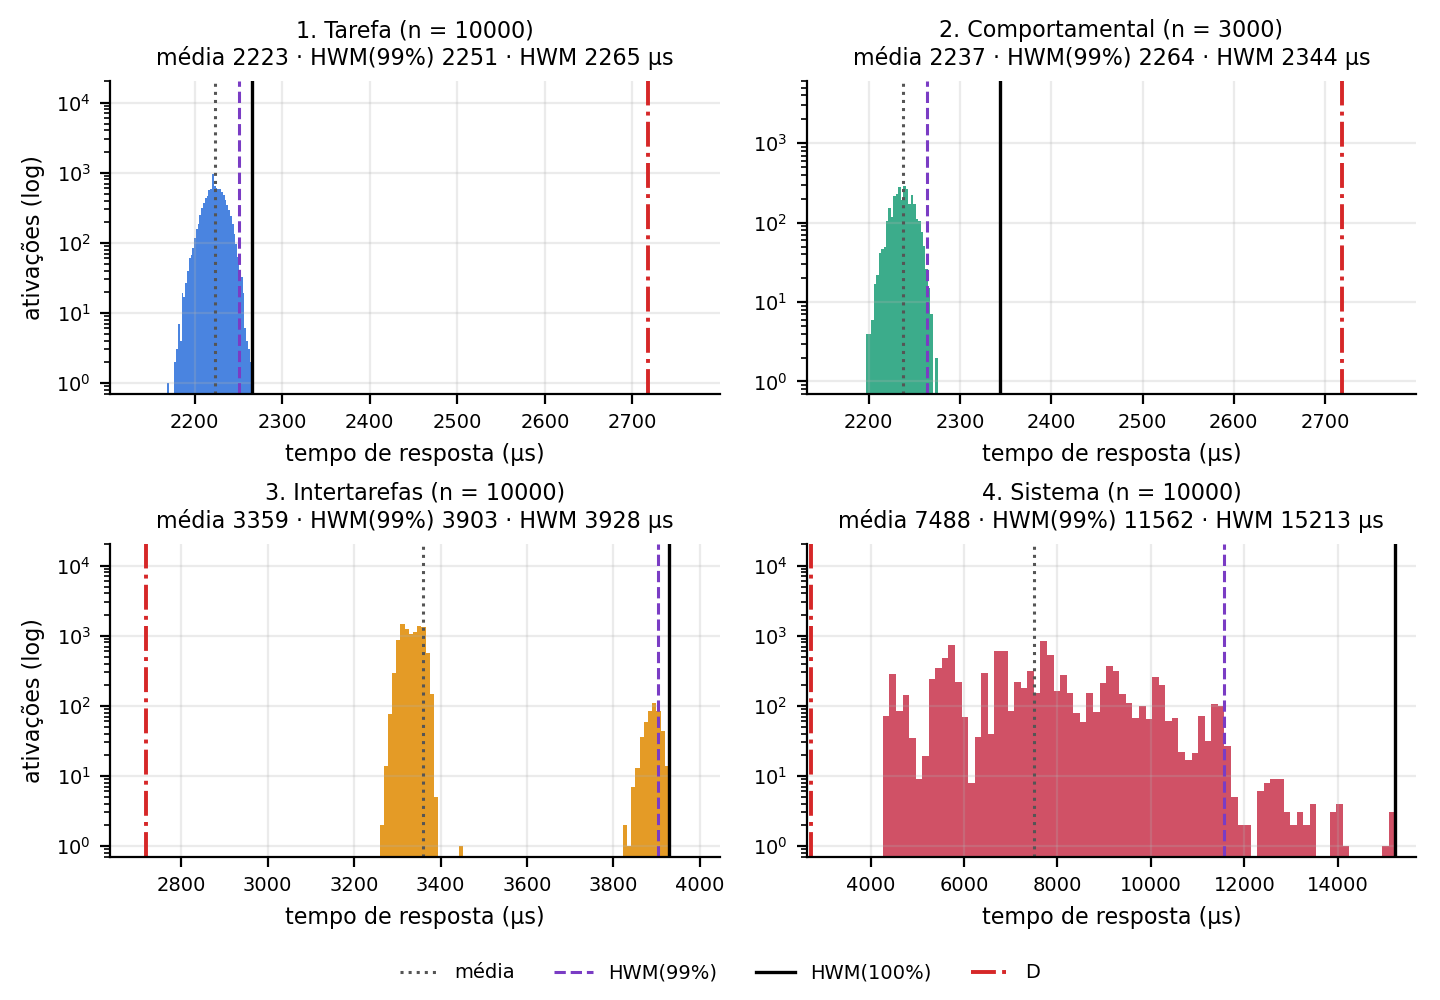
\includegraphics[width=0.56\textwidth]{figuras/esp32_fig1_histogramas.png}
\caption{Histogramas do tempo de resposta (contagem em escala logarítmica), com
média, HWM(99\%), HWM(100\%) e $D$.}
\label{fig:hist}
\end{figure}

Nas etapas 1 e 2, quase todos os tempos ficam entre 2.193 e 2.251\us{} (p1 e
p99 da etapa 1), com desvio-padrão de 13 e 12\us. A cauda é curta: o HWM fica
14\us{} acima do HWM(99\%) na etapa 1 e 80\us{} na etapa 2. Na etapa 3, o tempo
mínimo já passa de $D$ e a distribuição tem dois grupos, um perto de 3,3\ms{} e
outro perto de 3,9\ms, com 3,0\% das ativações. Na etapa 4, a distribuição é
larga: p1 e p99 valem 4,41 e 11,56\ms, o desvio-padrão é de 1.769\us{} (CV de
23,6\%) e a cauda chega a 15,2\ms. A média de 7.488\us{} fica longe do máximo e
não descreve esse espalhamento. Avaliado só pela etapa 1, o sistema pareceria
folgado (100\% no prazo, HWM 17\% abaixo de $D$), o ``erro clássico'' que o
enunciado manda evitar~\cite{enunciado}; as etapas 3 e 4 mostram que essa
conclusão estaria errada.

% ============================ 3 =======================================
\section{Evolução temporal, perdas e skip factor}
O HWM passou de 2.265\us{} na tarefa isolada para 2.344\us{} com o evento
externo, 3.928\us{} com as três tarefas e 15.213\us{} no sistema
(Figura~\ref{fig:temporal}). O HWM da etapa 2 ocorreu no primeiro evento,
quando o cache da flash ainda estava frio. Na etapa 3, os picos se repetem a
cada 33 ativações, que é o período com que a fase entre \textit{huffman}
(10\ms) e \textit{logger} (33\ms) se repete ($\mathrm{mmc} = 330$\ms); são as
ativações bloqueadas pelo mutex. Na etapa 4, o tempo oscila entre 4,4 e 11\ms{}
conforme a quantidade de bytes e de eventos que chegam durante cada ativação, e
os valores acima de 11,6\ms{} aparecem isolados ao longo de toda a etapa.

\begin{figure}[H]
\centering
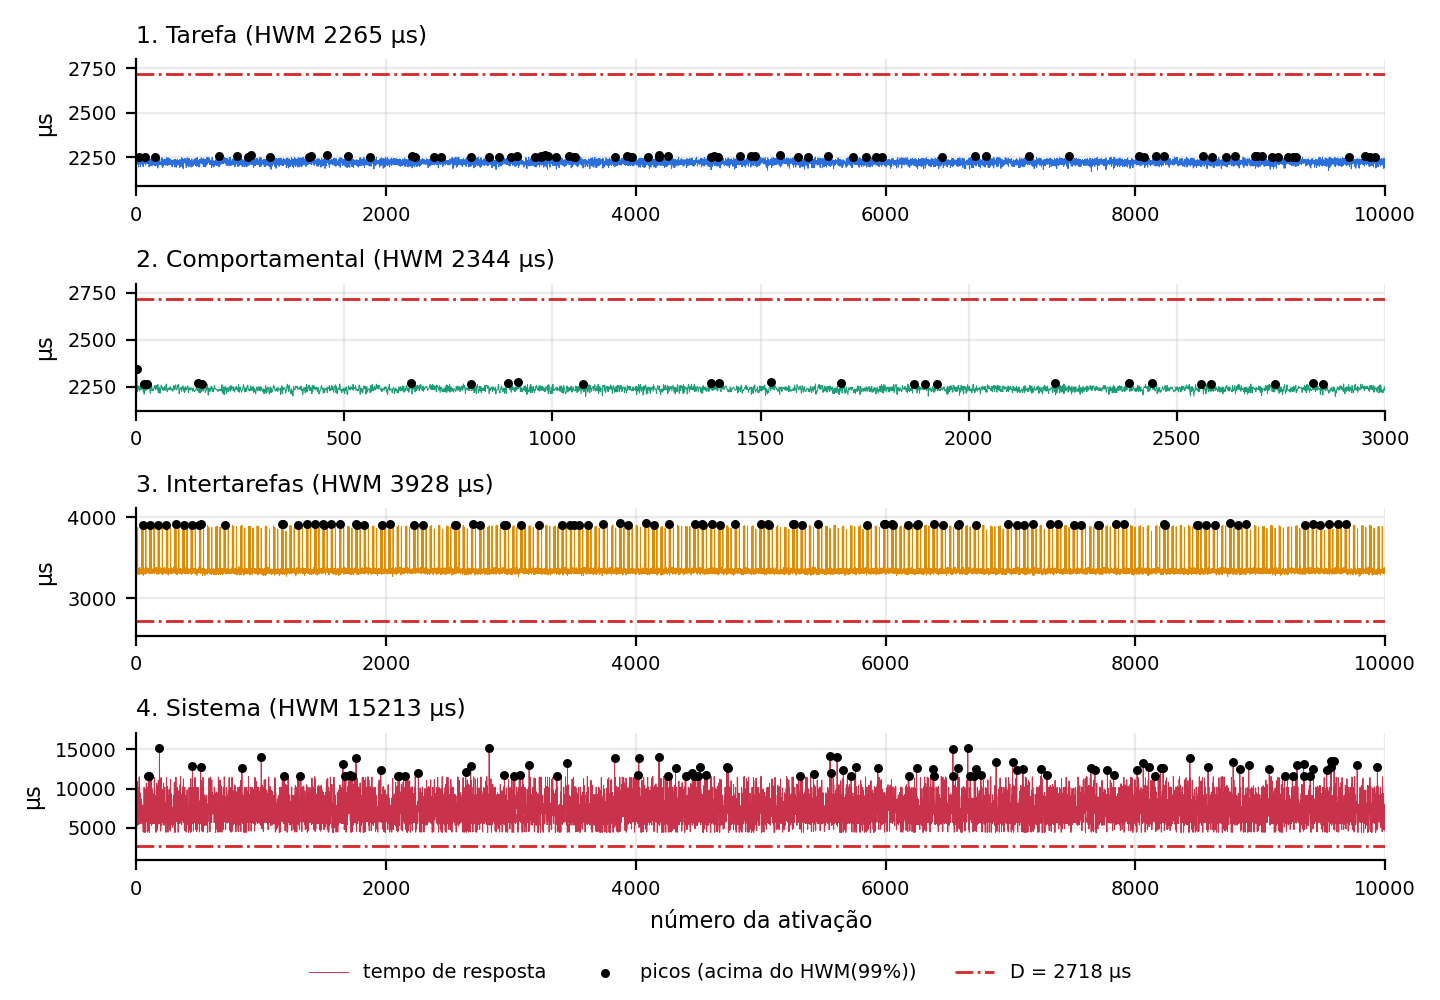
\includegraphics[width=0.56\textwidth]{figuras/esp32_fig2_temporal.png}
\caption{Tempo de resposta por ativação. Pontos marcados: valores acima do
HWM(99\%) da etapa; linha tracejada: $D$.}
\label{fig:temporal}
\end{figure}

\begin{table}[H]
\centering
\caption{Perdas com $D$ fixo. Uma sequência de tamanho 1 é uma perda isolada;
rajada é uma sequência de pelo menos duas perdas seguidas.}
\label{tab:perdas}
\small
\begin{tabular}{@{}lccccccc@{}}
\toprule
Etapa & N & Perdas & Prazo (\%) & Isoladas & Rajadas & Maior seq. & $S$ \\
\midrule
1 & 10.000 & 0      & 100,00 & 0 & 0 & 0      & -- \\
2 & 3.000  & 0      & 100,00 & 0 & 0 & 0      & -- \\
3 & 10.000 & 10.000 & 0,00   & 0 & 1 & 10.000 & 1 \\
4 & 10.000 & 10.000 & 0,00   & 0 & 1 & 10.000 & 1 \\
\bottomrule
\end{tabular}
\end{table}

Nas etapas 3 e 4, a lista de perdas é 1, 2, 3, \dots, 10.000, todas as
distâncias entre perdas valem 1, $S = 1$ e há uma única rajada com as 10.000
ativações. As listas completas estão em \texttt{results/esp32\_perdas\_etapaN.txt}.
Na etapa 3 a causa é a preempção pelo \textit{sensor}. O Huffman dura cerca de
2,2\ms{} e a defasagem entre as liberações do \textit{huffman} (múltiplos de
10\ms) e do \textit{sensor} (múltiplos de 4\ms) vale 0 ou 2\ms; portanto toda
ativação é interrompida uma vez pelo \textit{sensor}. Esse custo, de cerca de
1,0\ms, foi medido pela diferença entre as latências de início nas duas fases
(1.056 e 48\us). Ele é maior que os 250\us{} nominais porque o \textit{sensor}
gera dados com aritmética de 64 bits, emulada em software no Xtensa. Com isso,
o mínimo da etapa 3 (3.266\us) já passa de $D$. Na etapa 4, o registro de
detalhe mostra latência de início média de 1,15\ms{} (máximo de 6,6\ms),
execução média de 6,24\ms{} contra 2,2\ms{} isolada e bloqueio máximo de
5,95\ms, contra 0,59\ms{} na etapa 3, porque as interrupções da UART também
alongam a seção crítica do \textit{logger}.

% ============================ 4 =======================================
\section{Análise específica de \texorpdfstring{$(m,k)$}{(m,k)}-firme}
\label{sec:mk}
Uma tarefa é $(m,k)$-firme quando cumpre pelo menos $m$ prazos em qualquer
janela de $k$ ativações seguidas~\cite{hamdaoui,bernat}. Para $k = 10$, 20 e
50, foram percorridas todas as $N - k + 1$ janelas completas, avançando uma
ativação por vez. Sendo $L$ o número de perdas na pior janela, $m = k - L$
(função \texttt{miss\_analysis} em \texttt{analysis/analyze.py}).

Nas etapas 1 e 2, nenhuma janela tem perda, e os resultados são $(10,10)$,
$(20,20)$ e $(50,50)$. Nas etapas 3 e 4, todas as janelas estão cheias de
perdas, e os resultados são $(0,10)$, $(0,20)$ e $(0,50)$
(Figura~\ref{fig:janela}). Ou seja, com o $D$ tirado do teste isolado, o
sistema integrado não atende nenhum requisito $(m,k)$. Para que a análise
diga algo útil, $D$ tem de ser escolhido a partir do escopo de sistema, o que é
feito no Experimento D (Seção~\ref{sec:expD}).

\begin{figure}[H]
\centering
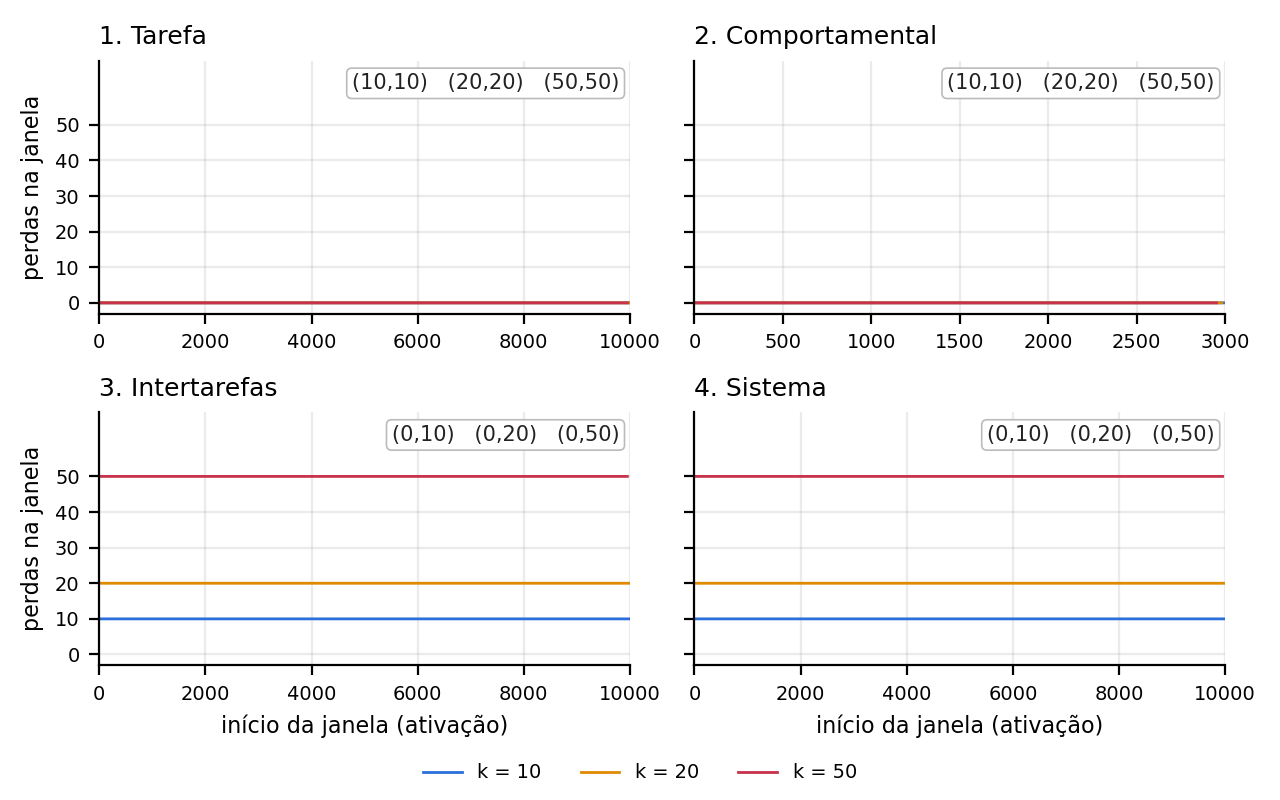
\includegraphics[width=0.58\textwidth]{figuras/esp32_fig4_janela.png}
\caption{Perdas em cada posição da janela deslizante ($k = 10$, 20 e 50) com
$D$ fixo; no canto de cada gráfico, o $(m,k)$ resultante.}
\label{fig:janela}
\end{figure}

\textbf{Limites.} O $(m,k)$ obtido dessa forma descreve apenas as 10.000
ativações medidas, com esta placa, este firmware e este estímulo. A janela só
examina sequências que de fato ocorreram; na etapa 4, o HWM ainda aumentou na
ativação 2.826, então pode existir uma janela pior que não foi amostrada. O
resultado também depende de $D$, de $k$, da taxa da UART, dos intervalos dos
eventos e da fase entre as tarefas. Não é prova de escalonabilidade nem
garantia para execuções futuras, que exigiria análise formal~\cite{bernat}. O
uso prático é como critério de aceitação que pode ser conferido em cada nova
campanha, por exemplo ``nenhuma janela de 20 ativações com mais de duas
perdas''.

% ============================ 5 =======================================
\section{Experimentos A, B e C}
\subsection{A -- Cobertura e HWM}
\label{sec:expA}
A cobertura foi medida com gcov/gcovr no PC, compilando com \texttt{-O0
--coverage} o mesmo \texttt{huffman.c} do firmware, com os mesmos casos e o
mesmo $N = 1.024$. No ESP32, o gcov exigiria depuração por JTAG, e a cobertura
depende apenas do código e das entradas. O HWM de cada caso foi medido no
ESP32, com 200 repetições.

\begin{table}[H]
\centering
\caption{Cobertura acumulada de \texttt{huffman.c} (143 linhas, 58 desvios) e
HWM de cada caso no ESP32.}
\label{tab:cobertura}
\small
\begin{tabular}{@{}lccc@{}}
\toprule
Casos (acumulados) & Linhas & Desvios & HWM (\textmu s) \\
\midrule
1 aleatório, $N = 1.024$         & 92,3\% & 86,2\% & 2.251 \\
+2 entrada vazia                 & 95,1\% & 91,4\% & 26 \\
+3 símbolo único                 & 99,3\% & 98,3\% & 423 \\
+4 dois símbolos                 & 99,3\% & 98,3\% & 583 \\
+5 256 símbolos com mesma frequência & 99,3\% & 98,3\% & 2.014 \\
+6 frequências de Fibonacci      & 99,3\% & 98,3\% & 1.029 \\
+7 saída corrompida              & 100\%  & 100\%  & 290 \\
\bottomrule
\end{tabular}
\end{table}

Com sete casos, a cobertura chegou a 100\% das linhas e dos desvios. A entrada
aleatória sozinha não passa pela entrada vazia, pelo símbolo único (árvore com
uma folha e código de 1 bit) nem pelo ramo de falha da validação, e todos os
casos que completam a cobertura são mais rápidos que ela. Quando a cobertura
chegou a 100\%, o HWM da etapa 1 era de 2.265\us. Nas etapas seguintes não há
caminho novo a percorrer, mas o HWM subiu para 2.344, 3.928 e 15.213\us. A
cobertura indica quais caminhos do código foram executados; o tempo de
resposta depende também de quando a tarefa roda e de quem disputa o
processador com ela (preempção, bloqueio, interrupções e estado do cache), e
isso não aparece no grafo de controle de \texttt{huffman.c}. A ativação de
15,2\ms{} passa pelos mesmos caminhos que uma de 2,2\ms. Os dados confirmam
que cobrir 100\% dos caminhos não garante encontrar o WCRT.

\subsection{B -- Convergência}

\begin{figure}[H]
\centering
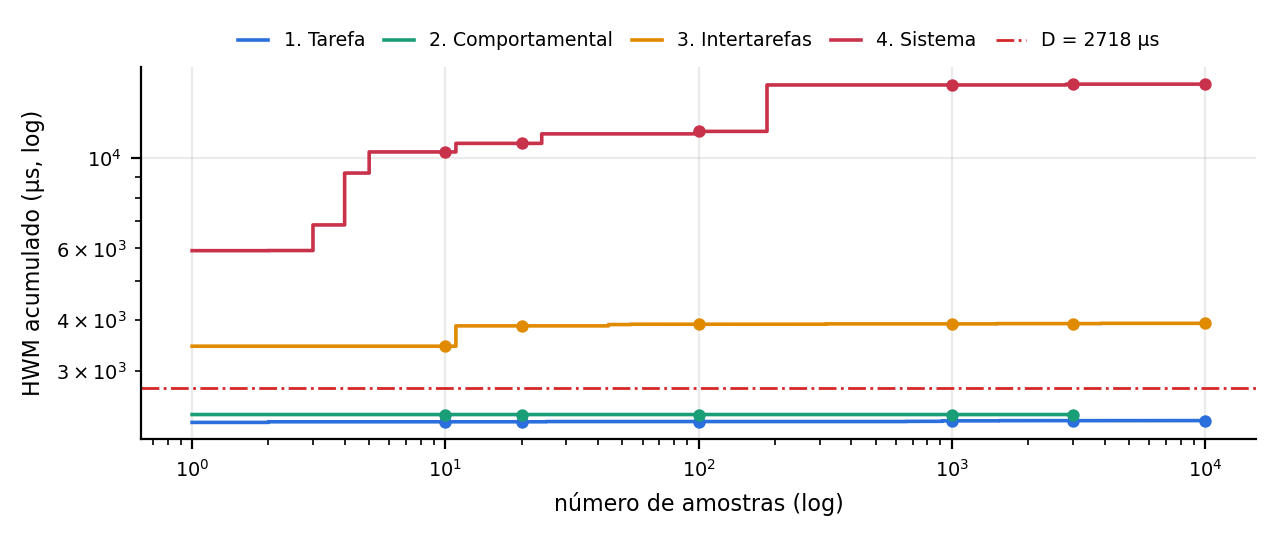
\includegraphics[width=0.55\textwidth]{figuras/esp32_fig3_convergencia.png}
\caption{HWM acumulado em função do número de amostras (escala log-log).}
\label{fig:conv}
\end{figure}

\begin{table}[H]
\centering
\caption{HWM acumulado (\textmu s) por número de amostras.}
\label{tab:conv}
\footnotesize
\setlength{\tabcolsep}{4pt}
\begin{tabular}{@{}lccccccccc@{}}
\toprule
Etapa & 10 & 20 & 100 & 1.000 & 3.000 & 10.000 & Saltos & Último salto & 95\% do final \\
\midrule
1 & 2.250  & 2.250  & 2.253  & 2.262  & 2.264  & 2.265  & 8  & 4.186 & 1 \\
2 & 2.344  & 2.344  & 2.344  & 2.344  & 2.344  & --     & 1  & 1     & 1 \\
3 & 3.451  & 3.872  & 3.908  & 3.916  & 3.922  & 3.928  & 8  & 3.872 & 11 \\
4 & 10.364 & 10.879 & 11.642 & 15.142 & 15.213 & 15.213 & 11 & 2.826 & 186 \\
\bottomrule
\end{tabular}
\end{table}

Nas etapas 1 a 3, o HWM estabiliza cedo (Figura~\ref{fig:conv}). Há saltos
tardios, como o da ativação 4.186 na etapa 1, mas eles somam só 0,7\% do
valor. Com 10 amostras, o HWM já estaria a menos de 2\% do final na etapa 1 e
a 12\% na etapa 3. Na etapa 4, com 10 amostras o HWM seria de 10,4\ms, 32\%
abaixo do valor final de 15,2\ms. O maior salto (de 11,6 para 15,1\ms)
acontece entre as amostras 100 e 1.000, e o último, na ativação 2.826. Com 10
ou 20 amostras, o sistema pareceria bem mais rápido do que é. Depois da
ativação 2.826 o HWM não mudou, mas isso não prova que ele chegou ao WCRT.

\subsection{C -- Margens de segurança}

\begin{table}[H]
\centering
\caption{Margens sobre o HWM(100\%) da etapa 1 (2.265\us).}
\label{tab:margens}
\small
\begin{tabular}{@{}cccccc@{}}
\toprule
Margem & Limite (\textmu s) & Etapa 2 & Etapa 3 & Etapa 4 & HWM4 $-$ limite (\textmu s) \\
\midrule
10\% & 2.492 & cobre & não cobre & não cobre & 12.721 \\
25\% & 2.831 & cobre & não cobre & não cobre & 12.382 \\
50\% & 3.398 & cobre & não cobre & não cobre & 11.815 \\
\bottomrule
\end{tabular}
\end{table}

As três margens cobrem a etapa 2, que precisaria de 3,5\%, e falham a partir
da etapa 3, que precisaria de 73,4\%; a etapa 4 precisaria de 572\%. Com a
margem de 50\%, 95,45\% das ativações da etapa 3 ficam abaixo do limite, mas o
HWM não. O desvio-padrão sobe de 13\us{} na etapa 1 para 118\us{} na etapa 3 e
1.769\us{} na etapa 4, e uma margem fixa calculada no teste isolado não
acompanha essa mudança. É a situação do exemplo da aula~\cite{aula}, com
tarefas que variam entre 12 e 14\ms{} e entre 10 e 16\ms: as médias são
parecidas, mas a margem que serve para a primeira não serve para a segunda. Na
etapa 3 a variação ainda é pequena (CV de 3,5\%), e mesmo assim são necessários
73\%, porque o \textit{sensor} soma cerca de 1\ms{} a toda ativação.

A etapa 3 pode ser conferida pela análise de tempo de resposta,
$R = C + B + \sum_j \lceil R/T_j \rceil C_j$~\cite{liu,sha}. Com
$C = 2.265\us$, $B = 1.520\us$ (seção crítica do \textit{logger}) e o
\textit{sensor} com $C_j = 1.008\us$ e $T_j = 4\ms$, a iteração converge em
$R = 2.265 + 1.520 + 2 \times 1.008 = 5.801\us$. O HWM medido (3.928\us) fica
abaixo desse limite: a medição dá um limite inferior e a análise, um limite
superior. A diferença vem de combinações de fase que não ocorreram (o maior
bloqueio observado foi de 587\us).

% ============================ 6 =======================================
\section{Experimento D: deadlines alternativos}
\label{sec:expD}
As análises das Seções 3 e 4 foram repetidas nas etapas 3 e 4 para quatro
valores de $D$: o HWM(100\%) da etapa 1, o $D$ fixo, um valor intermediário
($7.140\us$) e o HWM(99\%) da etapa 4. Os resultados completos estão em
\texttt{results/esp32\_expD.csv}.

\begin{table}[H]
\centering
\caption{Deadlines alternativos. I/R/M = perdas isoladas / número de rajadas /
maior rajada.}
\label{tab:expD}
\footnotesize
\setlength{\tabcolsep}{3.6pt}
\resizebox{\textwidth}{!}{%
\begin{tabular}{@{}lcccccccccc@{}}
\toprule
& \multicolumn{3}{c}{Etapa 3} & \multicolumn{7}{c}{Etapa 4} \\
\cmidrule(lr){2-4}\cmidrule(l){5-11}
$D$ (\textmu s) & Prazo (\%) & $S$ & $k{=}20$ & Prazo (\%) & $S$ & $k{=}10$ & $k{=}20$ & $k{=}50$ & I/R/M & Perdas \\
\midrule
2.265 (HWM etapa 1)    & 0,00   & 1  & (0,20)  & 0,00  & 1 & (0,10) & (0,20)  & (0,50)  & 0/1/10.000     & 10.000 \\
2.718 ($D$ fixo)       & 0,00   & 1  & (0,20)  & 0,00  & 1 & (0,10) & (0,20)  & (0,50)  & 0/1/10.000     & 10.000 \\
7.140 (intermediário)  & 100,00 & -- & (20,20) & 44,75 & 1 & (0,10) & (1,20)  & (11,50) & 1.267/1.258/15 & 5.525 \\
11.562 (HWM(99\%) etapa 4) & 100,00 & -- & (20,20) & 99,01 & 2 & (8,10) & (18,20) & (46,50) & 99/0/--        & 99 \\
\bottomrule
\end{tabular}}
\end{table}

\begin{figure}[H]
\centering
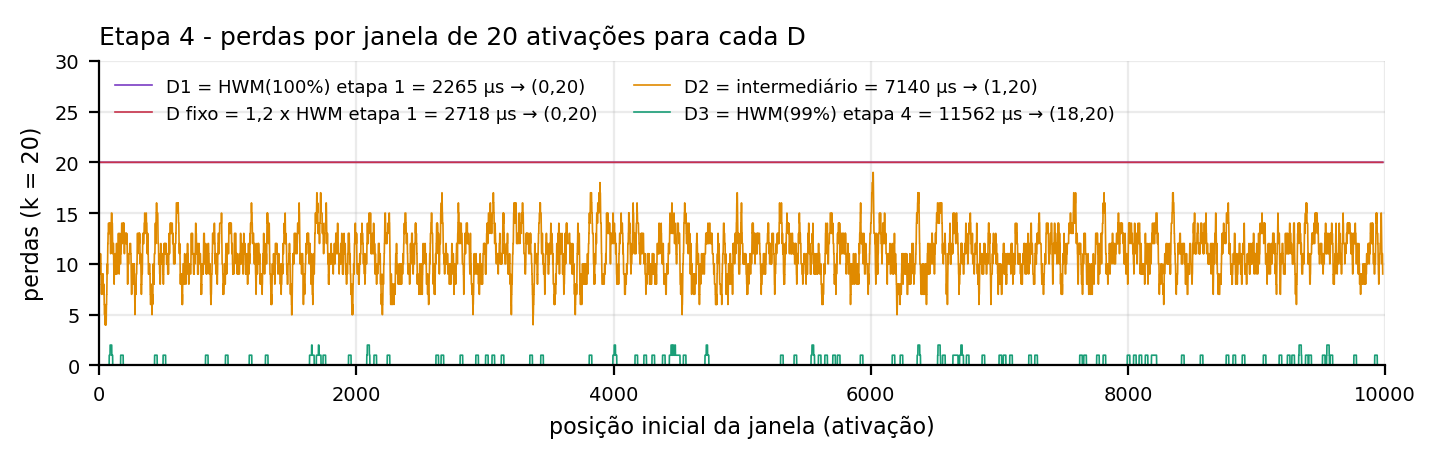
\includegraphics[width=0.52\textwidth]{figuras/esp32_fig7_expD_janela.png}
\caption{Perdas por janela de 20 ativações na etapa 4 para cada valor de $D$.}
\label{fig:expD}
\end{figure}

Na etapa 4, com $D = 7.140\us$, 55\% das ativações perdem o prazo: são 1.267
perdas isoladas e 1.258 rajadas, a maior com 15 perdas, e o resultado é
$(1,20)$. Com $D$ igual ao HWM(99\%), restam 99 perdas, todas isoladas, com
$S = 2$, e o resultado é $(18,20)$. Na etapa 3, a partir de $7.140\us$ não há
perdas.

\textbf{Menor $D$ para um $(m,k)$ exigido.} Como o número máximo de perdas por
janela só diminui quando $D$ aumenta, foi feita uma busca binária sobre os
próprios tempos medidos (função \texttt{min\_D\_for}). Na etapa 4, o menor $D$
é de 9.236\us{} para $(10,20)$, 10.435\us{} para $(15,20)$, 11.508\us{} para
$(18,20)$ e 12.805\us{} para $(19,20)$. Comparado com $D = $ HWM(100\%) $=
15.213\us$, exigir $(18,20)$ permite um prazo 24\% menor. Na etapa 3, $(18,20)$
exige 3.387\us{} e $(19,20)$ exige 3.916\us, praticamente o próprio HWM, porque
ali os picos são periódicos.
A meta $(18,20)$ é ilustrativa, já que o enunciado não define uma tolerância
física.

\textbf{Isoladas e rajadas.} Em um sistema com inércia física, como posição ou
temperatura, uma perda isolada tende a ser absorvida, porque a ativação
seguinte corrige o atraso. Perdas seguidas deixam o controle sem atualização
por vários períodos: a rajada de 15 perdas com período de 10\ms{} corresponde a
150\ms{} sem resposta. Por isso a distância entre perdas importa mais que o
percentual. Com $D$ igual ao HWM(99\%) de cada plataforma, ESP32 e Linux
cumprem 99\% dos prazos, mas o ESP32 tem só perdas isoladas, $(18,20)$,
enquanto o Linux tem rajadas de até nove perdas, $(8,20)$. O percentual não
separa os dois casos. A campanha não demonstra que essa tolerância seria segura
para um equipamento real.

% ============================ 7 =======================================
\section{Reprodutibilidade, limites e conclusão}
\subsection{Reprodutibilidade}
O repositório contém o firmware (\texttt{esp32/}), a tarefa
(\texttt{src/huffman.c}), os testes de cobertura (\texttt{tests/},
\texttt{scripts/coverage.sh}), os CSV brutos (\texttt{data/esp32/}) e os
scripts de análise. As tabelas e figuras são geradas a partir dos CSV com
\texttt{python3 analysis/analyze.py esp32}, de forma determinística. Uma nova
coleta (Seção~1.1) aplica o mesmo estímulo, mas os tempos podem variar; as
condições ficam registradas em \texttt{results/esp32\_plataforma.txt}.

\subsection{Comparação com Linux (opcional)}
\label{sec:linux}
As etapas foram repetidas em Linux 6.18 sob WSL2, em um Ryzen 5 5500X3D (6
núcleos, 12 threads), com o mesmo \texttt{huffman.c} e $N = 32.768$ para que o
tempo ficasse na mesma escala. A etapa 2 usa um evento UDP vindo de outro
processo, a etapa 3 usa SCHED\_FIFO e mutex com herança de prioridade, e a
etapa 4 acrescenta \texttt{stress-ng}. Havia 334 processos no Windows
hospedeiro, e o \textit{governor} não é acessível dentro da VM. Pela mesma
regra, $D = 1{,}2 \times 5.458 = 6.549\us$.

\begin{table}[H]
\centering
\caption{Síntese no Linux ($D = 6.549\us$). Tempos em \textmu s.}
\label{tab:linux}
\footnotesize
\setlength{\tabcolsep}{4pt}
\begin{tabular}{@{}lcccccccc@{}}
\toprule
Etapa & Mín. & Média & HWM(100\%) & HWM(99\%) & Prazo (\%) & $S$ & $k{=}20$ & Último salto \\
\midrule
1 & 1.491 & 1.581 & 5.458  & 1.956  & 100,00 & -- & (20,20) & 9.570 \\
2 & 1.548 & 1.743 & 4.719  & 2.043  & 100,00 & -- & (20,20) & 1.871 \\
3 & 1.535 & 1.838 & 5.847  & 2.605  & 100,00 & -- & (20,20) & 7.997 \\
4 & 1.552 & 3.195 & 69.551 & 10.744 & 96,25  & 1  & (2,20)  & 9.660 \\
\bottomrule
\end{tabular}
\end{table}

No Linux, o HWM já fica em 3,5 vezes a mediana na tarefa isolada (1,02 no
ESP32) e não estabilizou em nenhuma etapa. Na etapa 4, 68\% das perdas tiveram
latência de início acima de 500\us{} (máximo de 68\ms): a tarefa estava pronta
e não foi despachada, por causa do kernel sem PREEMPT\_RT e do hipervisor. No
ESP32, cada aumento do tempo tem uma causa identificável.

\subsection{Ameaças à validade}
\textbf{Plataforma e cache.} No ESP32 o código roda da flash por meio do cache,
cujo estado não foi controlado; o HWM da etapa 2 no primeiro evento é um
exemplo. O Linux é uma plataforma de propósito geral em VM, sem limite de
latência. Os valores absolutos não valem para outras placas.
\textbf{Energia e interrupções do SO.} A frequência do ESP32 é fixa, mas o tick
do FreeRTOS e o timer de liberação (1\,kHz cada) continuam ativos no núcleo 1.
\textbf{Instrumentação.} São duas leituras de relógio por ativação; os dados
ficam em RAM pré-alocada e só são enviados no fim da etapa.
\textbf{Estresse não coberto.} Não foram testados UART acima de 115.200 baud,
Wi-Fi nem gravação em flash; em um ensaio preliminar com flash e Wi-Fi, o HWM
chegou a 75,9\ms. \textbf{Amostragem.} Há uma campanha por etapa, com uma
semente e um tamanho de entrada; com 10.000 ativações, o pior caso real pode
ser maior que o medido.

\subsection{Conclusão}
O HWM passou de 2.265\us{} na tarefa isolada para 15.213\us{} no sistema (6,7
vezes), sempre pelos mesmos caminhos de um código com 100\% de cobertura de
linhas e desvios. O aumento vem da concorrência: preempção, bloqueio,
interrupções e cache, que só aparecem nos escopos intertarefas e de sistema.
Por isso o $D$ tirado da tarefa isolada foi perdido em todas as ativações das
etapas 3 e 4, e nenhuma das margens fixas cobriu a etapa 3: medir apenas a
tarefa isolada levaria ao erro clássico.

Como o WCRT não pode ser medido com certeza, o modelo $(m,k)$-firme dá um
critério que pode ser conferido janela a janela. Com os dados, foi possível
calcular o menor $D$ para cada requisito, por exemplo 11,5\ms{} para $(18,20)$,
24\% abaixo do HWM, e distinguir situações que o percentual de acertos não
separa: perdas isoladas no ESP32 e rajadas no Linux, ambos com 99\%. O
$(m,k)$ medido descreve o que foi observado e precisa ser conferido de novo a
cada campanha.

% ========================== REFERÊNCIAS ================================
\renewcommand{\refname}{Referências}
\begin{thebibliography}{9}
\setlength{\itemsep}{0pt}
\footnotesize

\bibitem{enunciado} UNIVALI. \textit{Atividade Complementar: Quanto o teste
enxerga do pior caso?} Sistemas em Tempo Real, M3. Enunciado fornecido na
disciplina, 2026.

\bibitem{aula} UNIVALI. \textit{Estimação do Tempo de Resposta usando
Medições.} Sistemas em Tempo Real. Material de aula fornecido na disciplina,
2026.

\bibitem{huffman} HUFFMAN, D. A. A method for the construction of
minimum-redundancy codes. \textit{Proceedings of the IRE}, v.~40, n.~9,
p.~1098--1101, 1952.

\bibitem{liu} LIU, C. L.; LAYLAND, J. W. Scheduling algorithms for
multiprogramming in a hard-real-time environment. \textit{Journal of the ACM},
v.~20, n.~1, p.~46--61, 1973.

\bibitem{sha} SHA, L.; RAJKUMAR, R.; LEHOCZKY, J. P. Priority inheritance
protocols: an approach to real-time synchronization. \textit{IEEE Transactions
on Computers}, v.~39, n.~9, p.~1175--1185, 1990.

\bibitem{hamdaoui} HAMDAOUI, M.; RAMANATHAN, P. A dynamic priority assignment
technique for streams with $(m,k)$-firm deadlines. \textit{IEEE Transactions on
Computers}, v.~44, n.~12, p.~1443--1451, 1995.

\bibitem{bernat} BERNAT, G.; BURNS, A.; LLAMOSÍ, A. Weakly hard real-time
systems. \textit{IEEE Transactions on Computers}, v.~50, n.~4, p.~308--321,
2001.

\bibitem{espidf} ESPRESSIF SYSTEMS. \textit{ESP-IDF Programming Guide}.
Disponível em: \url{https://docs.espressif.com/projects/esp-idf}. Acesso em:
18 nov. 2026.

\end{thebibliography}

\end{document}
